%======================================================================
\chapter{Background and Related Work}
%======================================================================

\section{Document Retrieval}

\subsection{Non-Neural Methods}

\subsection{Okapi BM25}

\myworries{Binary and its extension to BM25... shortcomings semantic}

Okapi BM25 (commonty dubbed BM25) is a bag-of-words ranking function that was developed to accommodate documents of variable lengths.
BM25 ranks documents based on the occurrence of query terms in each document, paying more attention to the rarer terms in the query.
The goal of this approach is to take into account term frequency and document frequency while estimating the relevance of a document for a given query without introducing too many additional parameters. (Sparck)
To achieve this goal, BM25 implementations define two parameters for term frequency saturation and field-length normalization, respectively.
\myworries{Tuned for most common datasets?}

\subsection{RM3}

RM3 is a pseudo-relevance feedback mechanism where the original query is expanded by adding terms found in the contents of relevant BM25 documents.
\myworries{Why is it effective, why does it improve performance, how common is it}

\myworries{Previous approaches and results on these datasets}

\subsection{Neural Methods}

\begin{figure}[t!]
\centering
  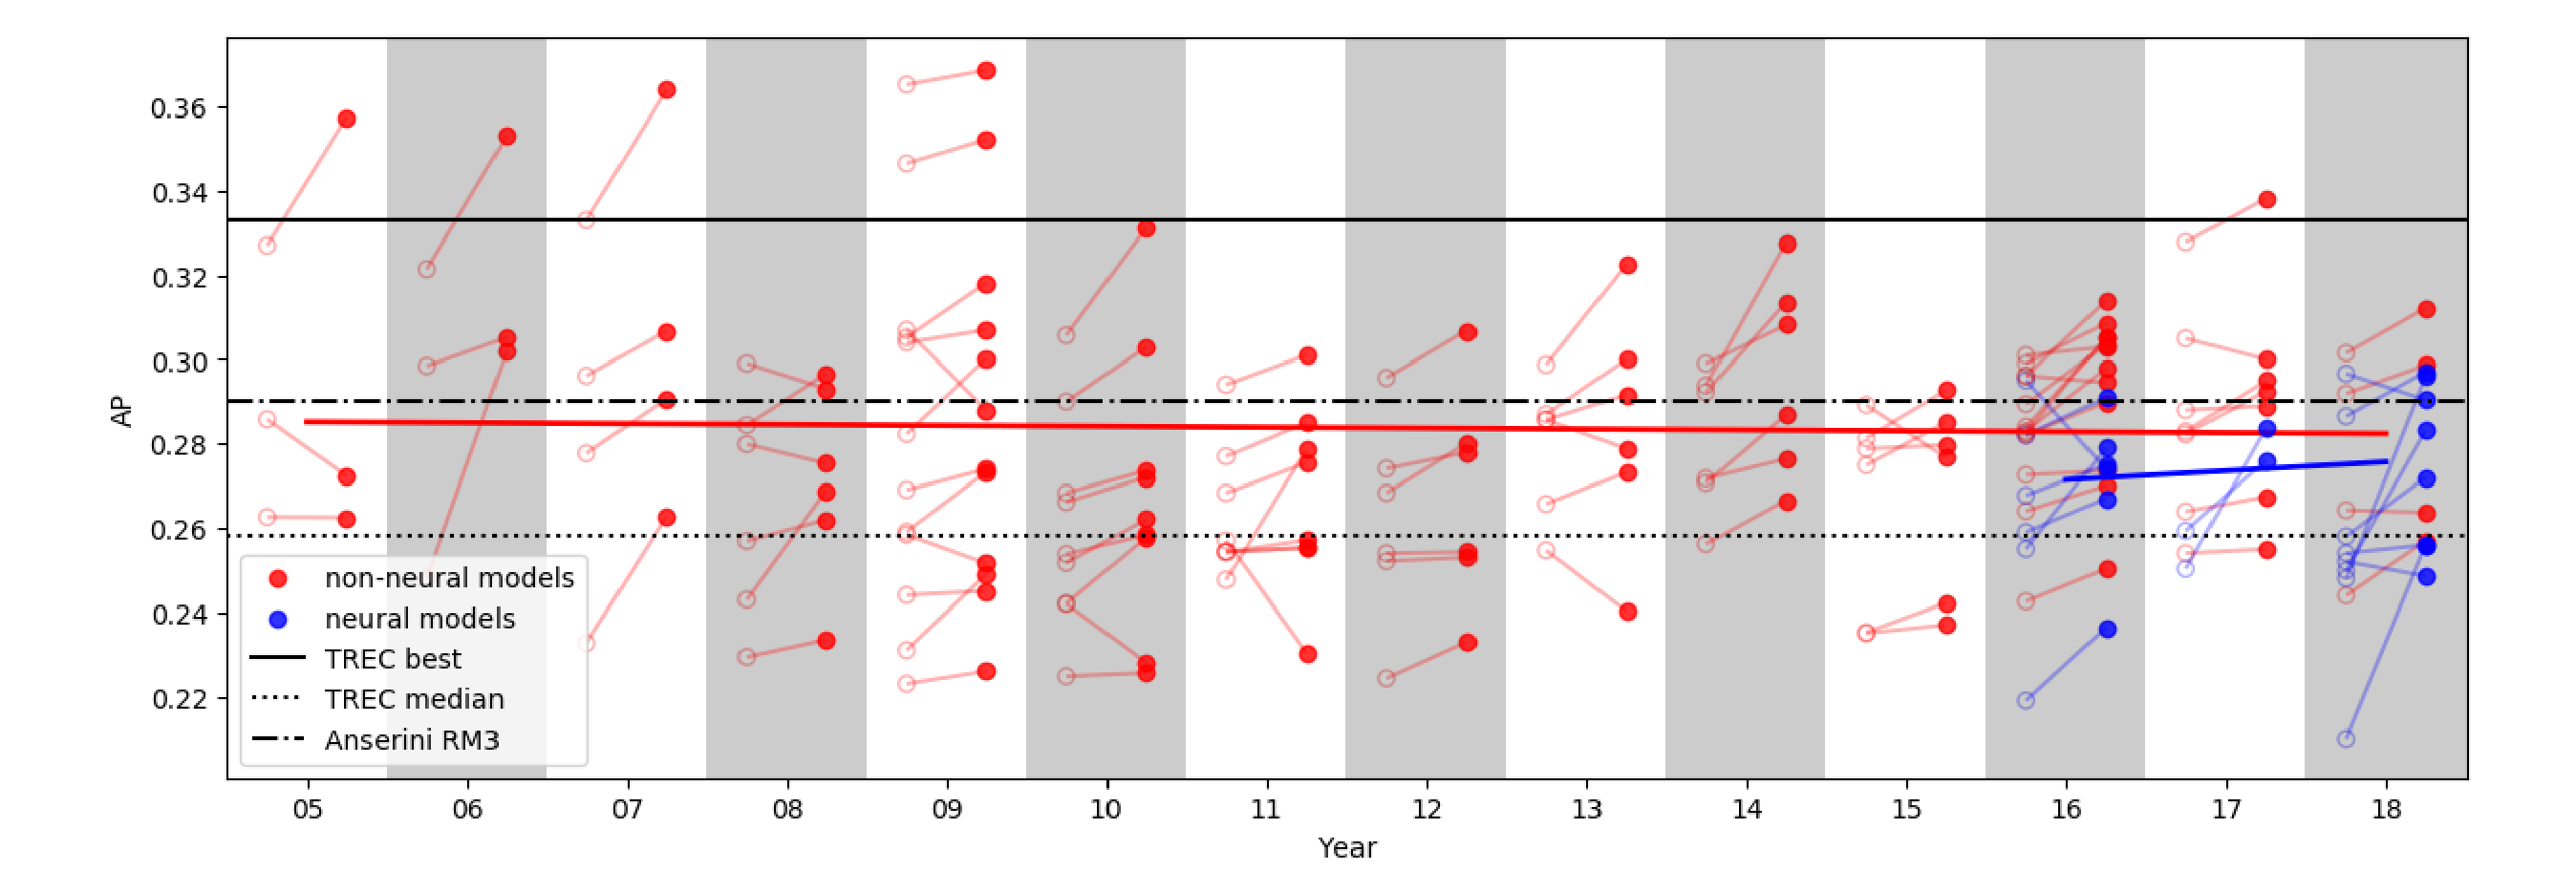
\includegraphics[width=7in]{neural_robust04.png}
\caption{.l.}
\label{fig:bert}
\end{figure}



%To be clear, our focus is on neural ranking models for {\it ad hoc} document retrieval, over corpora comprising news articles.
%Formally, in response to a user query $Q$, the system's task is to produce a ranking of documents from a corpus that maximizes some ranking metric---in our case, average precision (AP).
%We emphasize that this problem is quite different from web search, where there is no doubt that large amounts of behavioral log data, along with other signals such as the webgraph, have led to large improvements in search quality~\cite{MitraBhaskar_Craswell_2019}.
%Instead, we are interested in limited data conditions---what can be achieved with modest resources outside web search engine companies such as Google and Microsoft who have large annotation teams---and hence we only consider ``classic'' TREC newswire test collections.

%The dominant approach to {\it ad hoc} document retrieval using neural networks today is to deploy the neural model as a reranker over an initial list of candidate documents retrieved using a standard bag-of-words term-matching technique.
%Despite the plethora of neural models that have been proposed for document ranking, there has recently been some skepticism about whether they have truly advanced the state of the art~\cite{Lin_SIGIRForum2018}, at least in the absence of large amounts of behavioral log data only available to search engine companies.
%
%In a meta-analysis of over 100 papers that report results on the dataset from the Robust Track at TREC 2004 (Robust04), \cite{Yang_etal_SIGIR2019} found that most neural approaches do not compare against competitive baselines.
%To provide two recent examples, McDonald report a best AP score of 0.272 and Li 0.290, compared to a simple bag-of-words query expansion baseline that achieves 0.299.
%Further experiments by \cite{Yang_etal_SIGIR2019} achieve 0.315 under more rigorous experimental conditions with a neural ranking model, but this is still pretty far from the best-known score of 0.3686 on this dataset~\cite{Cormack:2009:RRF:1571941.1572114}.
%
%Although Sculley remind us that the goal of science is not {\it wins}, but knowledge, the latter requires first establishing strong baselines that accurately quantify proposed contributions.
%Comparisons to weak baselines that inflate the merits of an approach are not new problems in information retrieval.
%...
%
%Having placed evaluation on more solid footing with respect to well-tuned baselines by building on previous work, this paper examines how we might make neural approaches ``work'' for document retrieval.
%One promising recent innovation is models that exploit massive pre-training ..., leading to BERT \cite{devlin2018bert} as the most popular example today.
%Researchers have applied BERT to a broad range of NLP tasks with impressive gains:\
%most relevant to our document ranking task, these include BERTserini for question answering and~\cite{nogueira2019passage} for passage reranking.

\section{Semantic Matching}

\myworries{Latent semantic models}

\myworries{Unsupervised language models}

\myworries{BERT}

\section{BERT}

\begin{figure}[b!]
\centering
  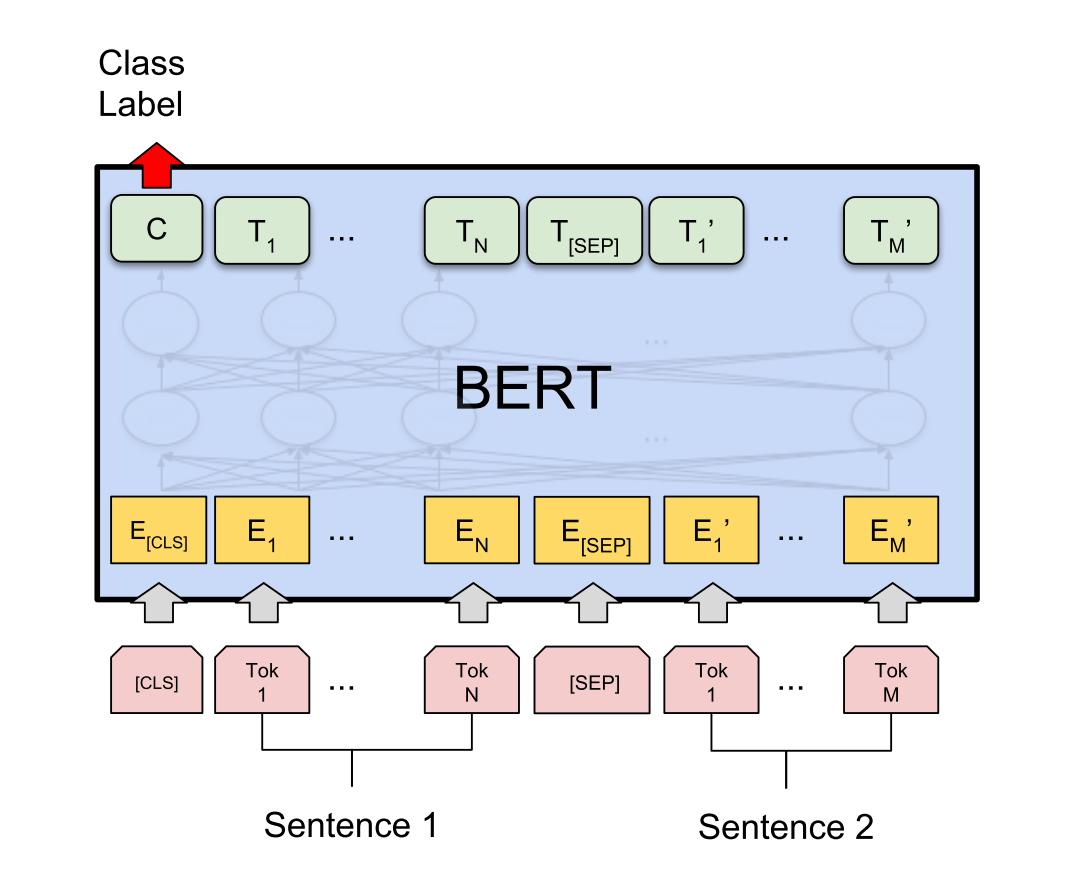
\includegraphics[width=5in]{classification.png}
\caption{BERT Sentence Pair Classification Model.}
\label{fig:bert}
\end{figure}

With the increasing availability of large corpora, pretrained deep language models have been rapidly gaining traction among NLP researchers.
Recent work in NLP has demonstrated that language model pretraining has proven extremely effective for many natural language processing tasks ranging from machine translation to reading comprehension.
One of the latest and most sophisticated pretrained deep language models is undoubtedly the Bidirectional Encoder Representations from Transformers (BERT), which has already enjoyed widespread popularity across the NLP community.~\cite{devlin2018bert}
Unlike previous language models, such as OpenAI's Generative Pretrained Transformer (GPT)~\cite{radford2019language}, BERT produces deep bidirectional representations by conditioning on both left and right context in all layers by employing a new pretraining objective called ``masked language model'' (MLM).
Conceptually, MLM randomly masks some of the tokens from the input with the goal of predicting the original token based only on its left and right context.

As expected, optimizing this objective requires a very complex model:\ for example, the larger BERT model requires around 340 million parameters be optimized.
In fact, training this model end-to-end takes four days to complete even on 16 high-end tensor processing units (TPUs)~\cite{devlin2018bert}.
Fortunately, there exists a technique to benefit from these models without having to train an entire model from scratch.
The most versatile and widely adopted approach to applying these neural models to downstream NLP tasks is based on ``freezing'' their last layer, and ``fine-tuning'' on external data for the specific task.
Not only does this approach introduce only a few task-specific parameters to optimize, but it also greatly boosts the performance of many NLP tasks given the rich semantic expressiveness introduced by the pretrained language model.
Figure \ref{fig:bert} visualizes the input and output for fine-tuning BERT for a ``sentence pair classification'' model.
To form an input, two sequences of tokens are concatenated with the meta-token $[SEP]$, i.e: separator, and prepended with $[CLS]$, corresponding to the ``class'' meta-token.
A single-layer neural network is added to the end of this network with the class label as the input, and subsequently trained for the specific downstream task.

\myworries{Success in other tasks}

\myworries{BERT document retrieval}

%Beyond our own previous work~\cite{yang2019simple}, which to our knowledge is the first reported application of BERT to document retrieval, there have been several other proposed approaches, including~\cite{} and unrefereed manuscripts~\cite{Qiao:1904.07531:2019,Padigela:1905.01758:2019}.

BERTserini \cite{Yang_etal_arXiv2019} combines the open-source information retrieval toolkit Anserini\footnote{https://github.com/castorini/anserini} with a BERT-based reader to identify answers from a large corpus of Wikipedia articles in an end-to-end fashion.
With this pipeline, the authors are able to achieve large improvements over previous question answering systems.
Although this work aims to solve an entirely different task, we incorporate a similar architecture in this project with success.

On the other hand, Nogueira et al. \cite{nogueira2019passage} propose to re-rank MS MARCO passages based on a simple re-implementation of BERT, outperforming the previous state of the art by 27\% in MRR@10 and replacing the top entry in the leaderboard of the MS MARCO passage retrieval task at the time of publication.
Our neural model is inspired by the BERT re-implementation described in this paper.

\section{Evaluation Metrics}

The standard approach to evaluation in information retrieval relies on the distinction between ``relevant'' and ``irrelevant'' documents with respect to an information need as expressed by a query.
A number of automatic evaluation metrics has been formalized for ranking tasks such as document retrieval.
These metrics rely on 
The size of most document collections makes it infeasible for humans to manually judge the relevance of all documents.
All relevant documents need to be labelled to prevent false negatives, i.e: treating documents which are in fact relevant as irrelevant.

\subsection{Mean Average Precision (MAP)}

Precision specifies what fraction of a set of retrieved documents is in fact relevant for a given query $ q $.
Precision can easily be extended to evaluate ranked retrieval results by ...
Average precision (AP) expresses the average of the precision values obtained for the set of top $ k $ documents for a query.
Support that $ D = \{d_1, ..., d_{m_j}\} $ is the set of all relevant documents for a query $ q_j $, then AP can be formulated as:

\begin{equation}
AP = \frac{1}{m_j} \sum^{m_j} _{k = 1} P(R_{jk})
\end{equation}

where $ R_{jk} $ represents the set of top $ k $ tanked retrieval results.

The respective AP for each query can be aggregated to obtain mean average precision (MAP) for the overall retrieval effectiveness in the form of a single-figure measure of quality across various recall levels:

\begin{equation}
MAP = \frac{\sum^{|Q|} _{j = 1} AP}{Q} = \frac{1}{Q} \sum^{|Q|} _{j = 1} \frac{1}{m_j} \sum^{m_j} _{k = 1} P(R_{jk})
\end{equation}

%\myworries{Meaning of MAP: To recapitulate, if the AP is 0.5, the relevant
%answer occurs at every second position. If the AP score is 0.3, the relevant answer occurs
%at every 3rd position and an AP score of 0.1 would mean that every 10th answer is correct.}

It has been show to have especially good discrimination and stability compared to other metrics, which makes it the ideal choice for large text collections \cite{manning2010introduction}.
It is hence one of the standard metrics among the TREC community.

\subsection{Precision at k (P@k)}

Unlike MAP which factors in precision at all recall levels, certain applications have a distinctly different notion for ranking quality.
Particularly in the case of web search, the user often only cares about the results on the first page or two, but not all of them.
This restriction essentially leads to measuring precision at fixed low levels of retrieved results, i.e: top $ k $ documents -- hence the name for metric ``precision at $ k $''.
On the one hand, it eliminates the need for any estimate of the size of the set of relevant documents.
However, it also produces the least stable out of all measures.
Moreover, precision at $ k $ does not average well because the total number of relevant documents for a query has a very strong influence on its value. 

\subsection{Normalized Discounted Cumulative Gain (NDCG@20)}

NDCG is uniquely useful in applications with a non-binary notion of relevance, e.g: a spectrum of relevance. 
Like precision at k, it is evaluated as a weighted sum over the top k search results, and normalized so that a perfect ranking yields NDCG equals 1.

\myworries{math stuff}

NDCG is a popular choice for systems with machine learning approaches.

\section{Datasets}

\myworries{Add statistics and examples}

\myworries{Elaborate on splits}

\subsection{Fine-Tuning}

%\subsubsection{TREC Microblog}
%
%\subsubsection{MS MARCO}
%
%\subsubsection{TREC CAR}

As discussed in Section \ref{intro}, applying BERT to document retrieval requires leveraging passage- or sentence-level relevance judgements fortuitously available in large text collections.
Since no such newswire collection currently exists, we train the BERT relevance classifier on three out-of-domain collections.

TREC Microblog datasets draw from the Microblog Tracks at TREC from 2011 to 2014, with topics (i.e., queries) and relevance judgments over tweets. We use the dataset prepared by Rao et al. (2019)
MS MARCO features user queries sampled from Bing’s search logs and passages extracted from web documents. Each query is associated with sparse relevance judgments by human editors. TREC CAR uses queries and paragraphs extracted from English Wikipedia: each query is formed by concatenating an article title and a section heading, and passages in that section are considered relevant.
This makes CAR, essentially, a synthetic dataset.

\subsection{Evaluation}

%\subsubsection{Robust04}
%
%\subsubsection{Core17}
%
%\subsubsection{Core18}

We conduct end-to-end document ranking experiments on three TREC newswire collections:\
the Robust Track from 2004 (Robust04) and the Common Core Tracks from 2017 and 2018 (Core17 and Core18). Robust04 comprises 250 topics, with relevance judgments on a collection of 500K documents (TREC Disks 4 and 5).
Core17 and Core18 have only 50 topics each; the former uses 1.8M articles from the New York Times Annotated Corpus while the latter uses around 600K articles from the TREC Washington Post Corpus.